\section{Market Research}
Public lighting is essential to the society quality of life, since it allows citizens to enjoy public spaces at night, providing greater security. “In 1417, the Mayor of London ordered all houses to hang lanterns outdoors after dark during the winter months. This marked the first organized public lighting.”  \cite{street_lighting_history}.

Currently, many countries are replacing the traditional street lights, \ac{hps} which is a gas-discharge lamp that uses sodium to produce light at a distinctively yellow-orange, monochromatic glow, with the smart LED street lighting. \ac{led} technology has lower maintenance cost and operation cost that the \ac{hps} lamps, and can generate savings of more than 60 percent of energy costs \cite{light_pollution}, allowing payback of the initial investment. From oil lamps to \ac{led} lamps, public lighting has become a more efficient, cheaper and less polluting way of lighting the streets.

\subsection{Market Definition}
Smart Street lighting is a rapidly growing lighting market, boosted by regulatory policies that encourage energy efficiency, \ac{iot} convergence and the drop of LED prices. This new concept of smart light post is also growing, implementing not only the smart management of street lights, but also features that go from basic LED replacement control, to traffic and video monitoring, environmental monitoring, and others.

Smart street lights represent a strategic infrastructure for smart city development, in particular, for video-surveillance services and autonomous driving. \cite{market_growth_2}

In figure \ref{fig:market_growth}, we can see the global growth rate for connected street lighting market, evidencing the high growth rate in Asia, and the largest market in North America.

\begin{figure}[ht]
	\centering
	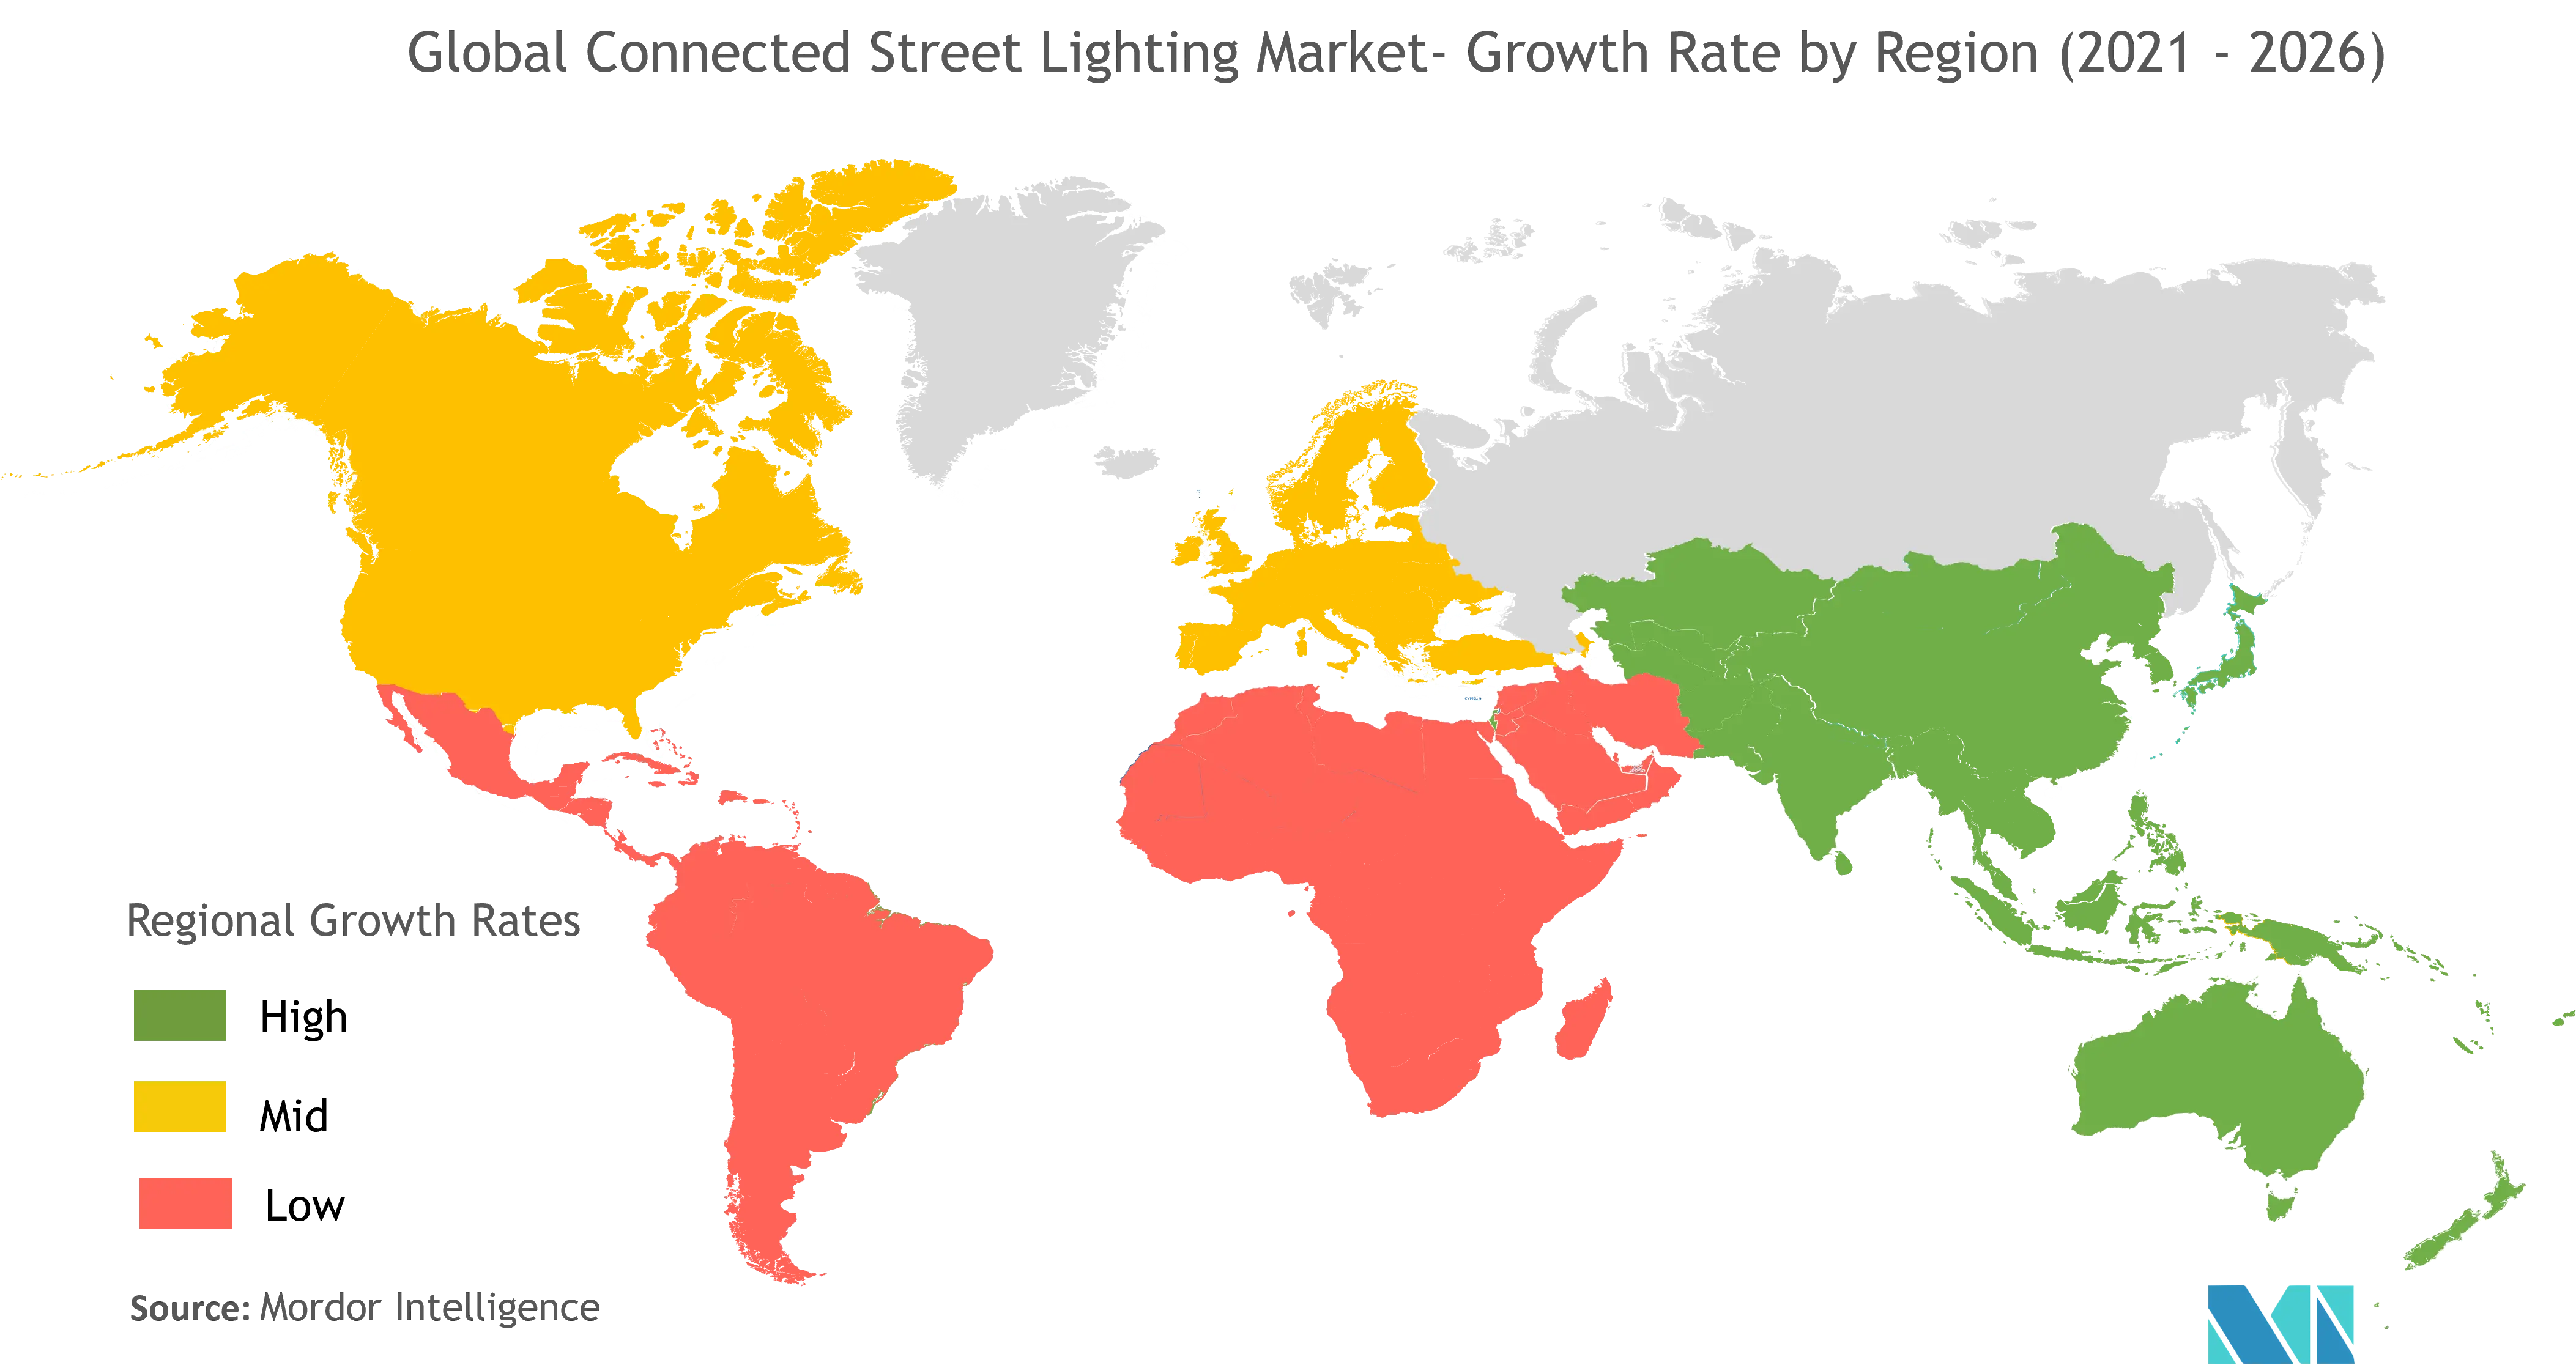
\includegraphics[width=1\textwidth]{market_growth_mordor}
	\caption{Global Connected Street Lighting Market - Growth Rate by Region \cite{market_growth}.}
	\label{fig:market_growth}
\end{figure}

\subsection{Scope}

In this project it will be implemented a street lighting solution for residential areas and public spaces, with the creation of smart light pole technology, feasible of being installed in existent lampposts, requiring minimum changes to the original infrastructure. This technology comprises sensors, a video-camera, a controller, and wireless connection to the smart street light network. This solution provides cost reduction and improved maintenance quality associated with street lighting, and also supports the deployment of smart city applications, through the use of the video-camera to detect available parking spaces.

\subsection{Similar products}

\subsubsection{Telensa - PLANet}

Nowadays, Telensa is the market share leader in smart street lighting with more than ten years of experience.\cite{telensa} PLANet is an intelligent street lighting system, consisting of wireless nodes connecting individual lights, a dedicated network owned by the city and a central management application, seen in figure \ref{fig:telensa}. This system reduces energy and maintenance costs associated with street lighting and also improves quality of maintenance through automatic fault reporting.

Doncaster, the largest metropolitan borough in England, houses over 45,000 smart Telensa streetlights, covering 220 square miles, achieving energy savings of approximately 1,5 million euros annually, with potential to increase this in the future.

Telensa is also developing a new generation of light pole sensor devices featuring smartphone \ac{ai} technology, enabling detailed real-time insights on traffic mix, pedestrian movements and others.

\begin{figure}[ht]
	\centering
	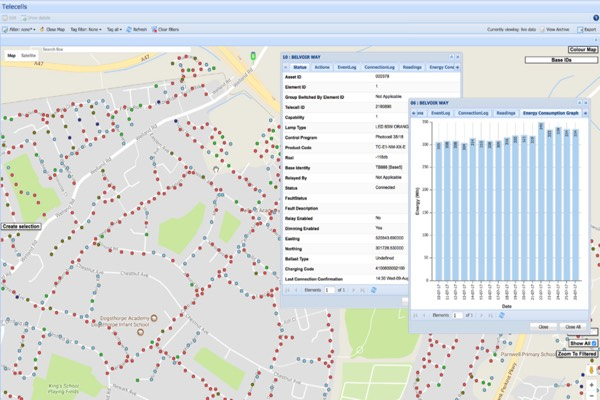
\includegraphics[width=0.8\textwidth]{telensa}
	\caption{Telecells - PLANet's Central Management System.}
	\label{fig:telensa}
\end{figure}


\subsubsection{FLASHNET - inteliLIGHT}
FLASHNET is a company focused on developing intelligent systems for smarter cities and better infrastructures and have created a solution that provides the right amount of light where and when needed to lighten the streets, the inteliLIGHT \cite{inteli_light}.

Using the existing infrastructure, this solution saves money and transforms the existing distribution level network into an intelligent infrastructure of the future, as shown in figure \ref{fig:intelilight}. Furthermore, the system is integrated with major \ac{iot} platforms and provides \ac{api} connectivity with City Management applications, ensuring compatibility with existing smart lighting and smart city initiatives.

\begin{figure}[ht]
	\centering
	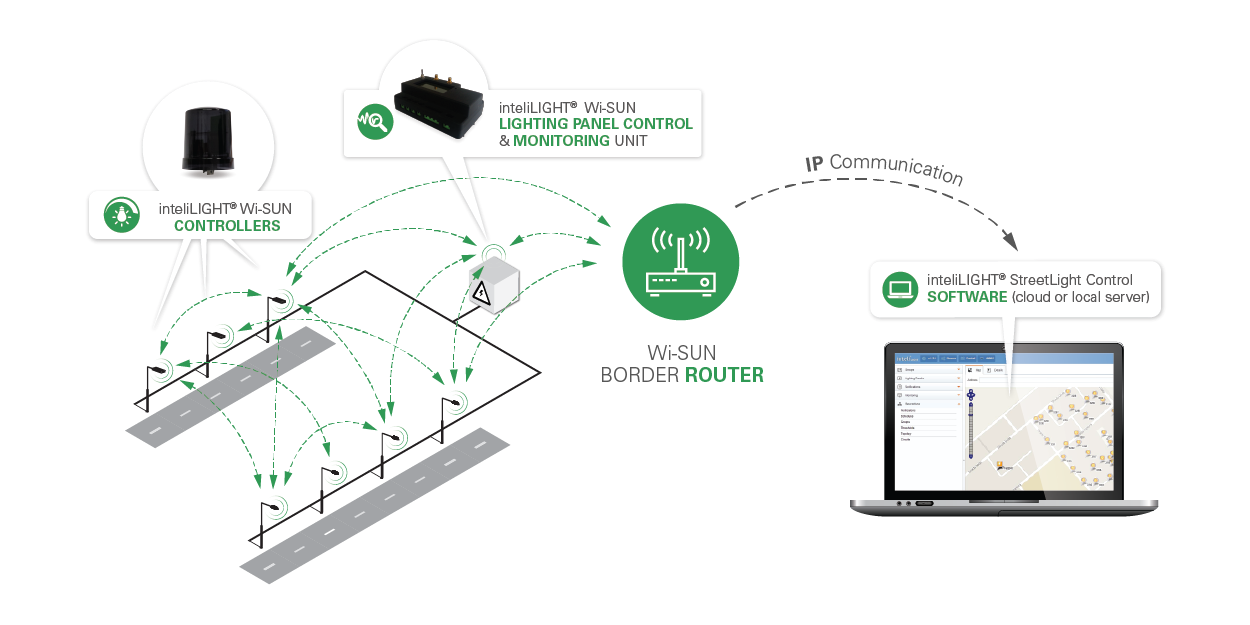
\includegraphics[width=0.95\textwidth]{intelilight}
	\caption{inteliLIGHT Communication Technology.}
	\label{fig:intelilight}
\end{figure}

\subsubsection{intuVision - intuVision VA Parking}
Regarding only to the detection of available parking spaces, there is a solution, by intuVision, named intuVision VA Parking, which provides parking lot analytics to determine vehicle count and security, and monitor parking space availability at all times, both for cities and for private parking lots, as one can see in the figure \ref{fig:intuvision}. \cite{parking}

\begin{figure}[ht]
	\centering
	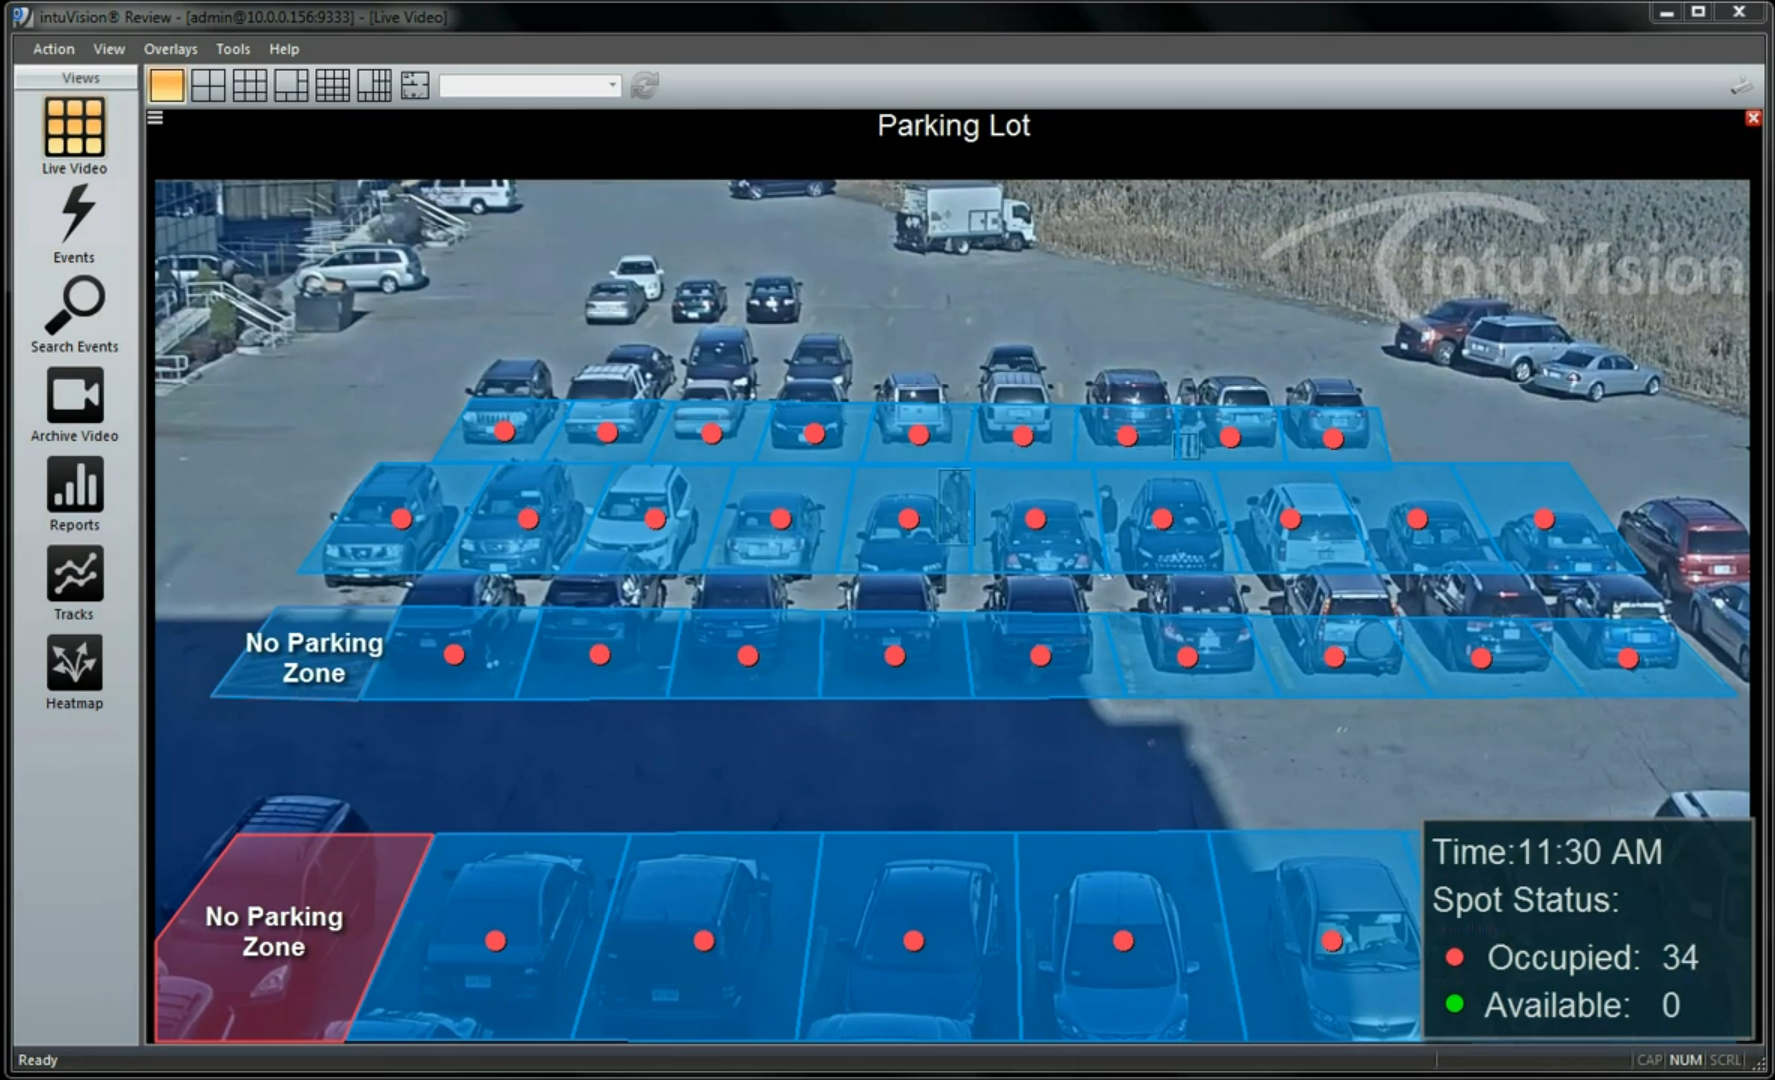
\includegraphics[width=0.8\textwidth]{intuvision}
	\caption{intuVision Parking Lot Demonstration.}
	\label{fig:intuvision}
\end{figure}

\subsection{Why choose our product}

This product aims to decrease power consumption associated with the traditional street light network, and also, using that infrastructure, contribute to the development of a smart city, detecting available parking spaces in the streets. It is a very scalable product, since each street lamp post connects to the rest of the network, via wireless, and one can monitor and process various areas of interest using the camera built in, aside the parking spaces availability detection. Besides the utilization in residential areas or public spaces, this can also be used in a large outdoor parking lot.